\documentclass{beamer}

\mode<presentation> {
\usetheme{Madrid}
}

\usepackage[utf8]{inputenc}
\usepackage[russian]{babel}
\usepackage{graphicx}
\usepackage{caption}
\usepackage{subcaption}
\usepackage{multimedia}
\usepackage{booktabs}

\author{Владислав Самсонов}
\title[MEMM]{Maximum-Entropy Markov Model}
\institute[MIPT]
{
Moscow Institute of Physics and Technology \\
\medskip
\textit{\href{mailto:vvladxx@yandex-team.ru}{vvladxx@yandex-team.ru}}
}
\date{November 27, 2016}

\newcommand\independent{\protect\mathpalette{\protect\independenT}{\perp}}
\def\independenT#1#2{\mathrel{\rlap{$#1#2$}\mkern2mu{#1#2}}}

\begin{document}

\begin{frame}
\titlepage
\end{frame}

%\begingroup
%\small
\begin{frame}{Maximum Entropy Markov Models}
\begin{block}{Дано}
Упорядоченная последовательность наблюдений (observations) $\{o_t\}_{t=1}^{n}:o_1, o_2, ..., o_n$ и \textbf{конечное} множество ответов $S$.\\
Примеры: текст, ДНК, значение амплитуды в момент времени $t$.
\end{block}
\begin{block}{Задача}
Присвоить каждому наблюдению $o_t$ ответ $s_t \in S$, максимизирующий условную вероятность $P(s_1,...,s_n|o_1,...,o_n)$:
$$\{s_1,...,s_n\}=\text{argmax}_{s_1,...,s_n} P(s_1,...,s_n|o_1,...,o_n)$$\\
Примеры: определить часть речи для слов из текста.
\end{block}
%\centerline{\includegraphics[width=6.8cm]{fig/interp-example.png}}
\end{frame}
%\endgroup

\begingroup
\small
\begin{frame}{Maximum Entropy Markov Models}
\begin{block}{Идея}
Заменить генеративную модель в HMM моделью максимальной энтропии.
\end{block}
\begin{block}{Maximum Entropy Markov Models}
Предположение о марковости: переходные вероятности зависят только от текущего наблюдения и прошлого ответа.
$$P(s_1,...,s_n|o_1,...,o_n) = \prod_{t=1}^{n} P(s_t | s_{t-1}, o_t)$$
\end{block}
\centerline{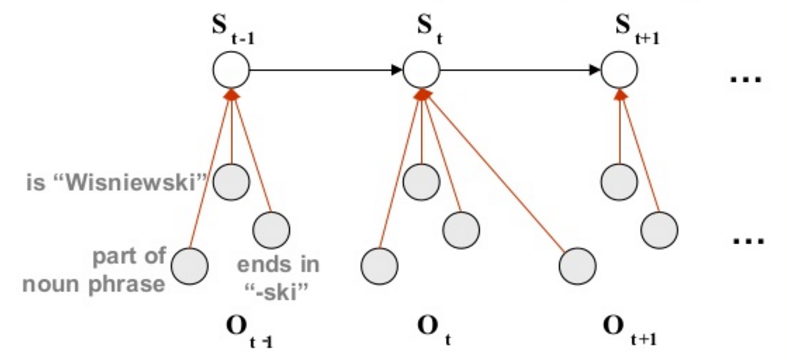
\includegraphics[width=6.2cm]{fig/memm.png}}
\end{frame}
\endgroup

\begin{frame}{MEMM vs HMM}
\begin{itemize}
\item HMM: максимиз. $P(s_1,...,s_n,o_1,...,o_n)=\prod_{t=1}^{n} P(s_t | s_{t-1}) P(o_t|s_{t-1})$
\item MEMM: максимизируем $P(s_1,...,s_n|o_1,...,o_n) = \prod_{t=1}^{n} P(s_t | s_{t-1}, o_t)$
\item HMM: пытаемся предсказывать наблюдения и ответы (но наблюдения нам известны, нужны только ответы).
\item MEMM: пытаемся предсказать только ответы.
\end{itemize}
\centerline{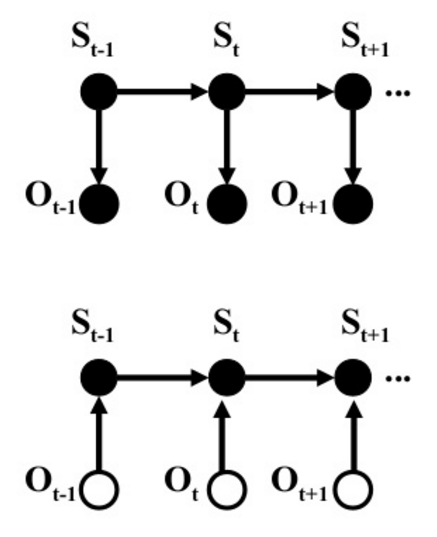
\includegraphics[width=3cm]{fig/hmmmemm.png}}
\end{frame}

\begin{frame}{MEMM vs HMM}
\centerline{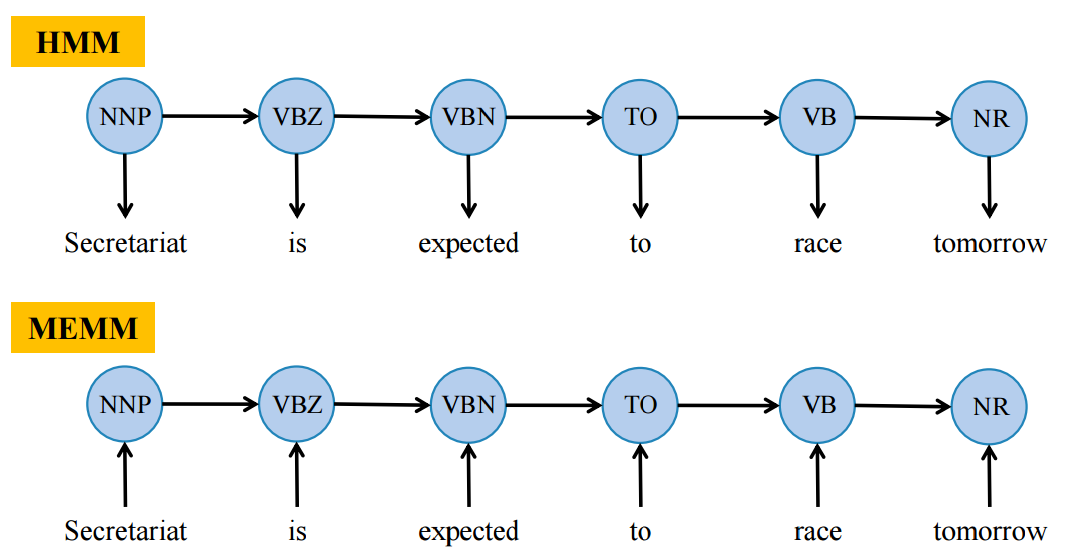
\includegraphics[width=10cm]{fig/hmmmemm1.png}}
\end{frame}

\begin{frame}{Недостатки HMM}
\begin{itemize}
\item Сильные предположения о данных: требуется незвисимость наблюдений $O\implies$ не учитываются взаимодействия между признаками (в MEMM нет такого предположения).
\item В каждом состоянии учитывается только одно наблюдение.
\item Размерность вектора $o_t \in O$ фиксирована.
\item Нет свободы в выборе признаков. На практике, при попытке учитывать сложные глобальные и даже локальные признаки сильно возрастает размерность вектора $o_t$.\\
Если попробовать учесть несколько соседних наблюдений вместо одного, то размерность растет.\\
Под глобальные признаки вроде количества точек в тексте нужно увеличивать размерность.
\end{itemize}
\end{frame}

\begin{frame}{Достоинства MEMM}
\begin{itemize}
\item Не требуется независимость наблюдений.
\item MEMM: прямое моделирование $P(s_t|s_{t-1},o_t)$ позволяет вычислить $P(s_1,...,s_n|o_1,...,o_n)$.
\item Количество наблюдений в момент времени $t$ может быть произвольным.
\end{itemize}
\centerline{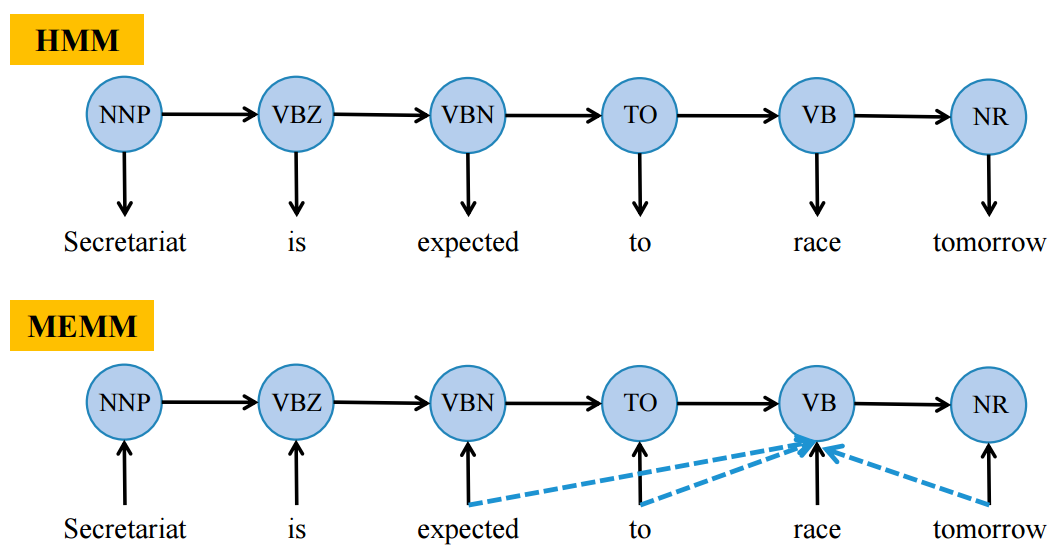
\includegraphics[width=10cm]{fig/hmmmemm2.png}}
\end{frame}

\begin{frame}{Недостатки MEMM}
\begin{itemize}
\item Семейства априорных распределений, которые можно использовать для $S$, не отличаются разнообразием.
\item Невозможно получить в некоторый момент времени вероятность произвольного наблюдения, т.к. мы изначально не учитывали это в модели. Есть возможность получить только вероятность ответа.
\end{itemize}
\end{frame}

\begin{frame}{Примеры признаков для MEMM}
\begin{columns}[c]
\column{.4\textwidth}
\begin{itemize}
\item Само слово.
\item Начинается ли с заглавной буквы.
\item Является ли ссылкой.
\item Является ли именем собственным.
\item Количество букв в слове.
\item Количество слов в тексте.
\item ...
\end{itemize}
\column{.6\textwidth}
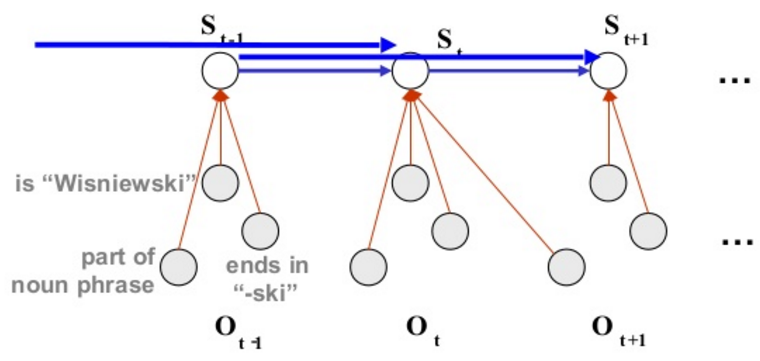
\includegraphics[width=7cm]{fig/memm1.png}
\end{columns}
\end{frame}

\begin{frame}{Проблемы}
Эмпирические оценки низкочастотных признаков ненадежны и могут приводить к переобучению.
Выбрасывание низкочастотных признаков не всегда помогает, т.к. эти признаки могут быть важны.\\
Решение: гауссовское сглаживание. Зададим априорное гауссовское распределение на параметры (оценка апостериорного максимума, maximum a posteriori estimation, MAP inference).
\centerline{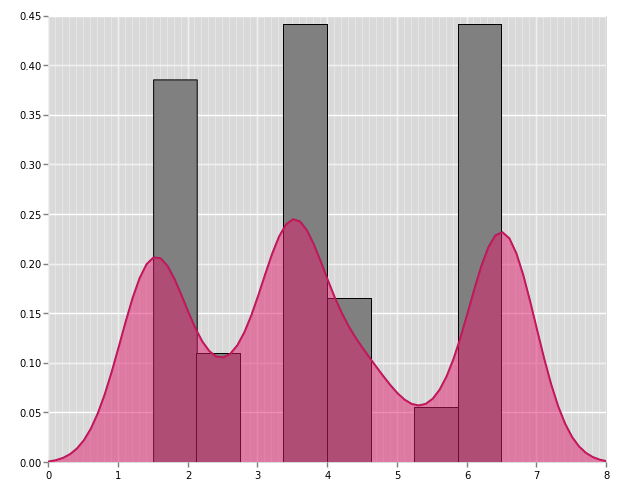
\includegraphics[width=6cm]{fig/gaussian_smoothing.png}}
\end{frame}

\begin{frame}{Метод максимальной энтропии}
Метод максимальной энтропии -- это метод для оценки распределения по данным.\\
Идея: принимаем гипотезу, которая максимизирует энтропию с дополнительными ограничениями.\\
Мотивация: распределение должно удовлетворять данным и делать как можно меньше предположений о данных (как можно ближе к равномерному распределению).
\end{frame}

\begin{frame}{Метод максимальной энтропии}
\begin{block}{Задача}
Хотим найти распределение, которое максимизирует энтропию при заданных линейных ограничениях.
\begin{equation*}
\begin{aligned}
& \underset{p}{\text{maximize}}
& & \left(-\sum_{x \in A \times B} p(x) \log p(x) \right) \\
& \text{subject to}
& & f_i(x) = c_i
\end{aligned}
\end{equation*}
\end{block}
\begin{block}{Идея решения}
Это задача нелинейного программирования с линейными ограничениями.\\
Применить метод множителей Лагранжа и теорему Каруша-Куна-Таккера $\implies$ получить задачу оптимизации без ограничений $\implies$ посчитать производную, приравнять 0 $\implies$ profit.
\end{block}
\end{frame}

\begin{frame}{Метод максимальной энтропии}
Закодируем все наблюдения $o_t$ с помощью бинарных предикатов: $b_t^i:O \rightarrow \{0,1\}$, где $i=1..B$.\\
Определим функции $f_t^i:O\times S \rightarrow \{0,1\}$ как
$$f_t^{i,s}(o_t,s_t) = \begin{cases} 1, & \mbox{если } b_t^i(o_t)=1\mbox{ и } s=s_t\\ 0, & \mbox{иначе}\end{cases}$$
Введём следующие ограничения:
$$\underset{(o_t,s_t) \sim Z}{\mathbb{E}} [f_t^{i,s}(o_t,s_t)] = \frac{1}{n} \sum_{t=1}^{n} f_t^{i,s}(o_t,s_t)$$
т.е. матожидание предиката в искомом распределении должно быть равно его выборочному среднему.
\end{frame}

\begin{frame}{Метод максимальной энтропии}
Итоговая задача оптимизации
\begin{equation*}
\begin{aligned}
& \underset{p}{\text{maximize}}
& & H(p) \\
& \text{subject to}
& & E^{i,s} = F^{i,s}
\end{aligned}
\end{equation*}
где
$$H(p)=- \frac{1}{n} \sum_{t=1}^{n} \sum_{s \in S} p(s|o_t) \log p(s|o_t)$$
$$E^{i,s} = \sum_{t=1}^{n} \sum_{s' \in S} p(o_t,s') f_t^{i,s}(o_t,s')$$
$$F^{i,s} = \frac{1}{n} \sum_{t=1}^{n} f_t^{i,s}(o_t,s_t)$$
\end{frame}

\begin{frame}{Метод максимальной энтропии}
Выписываем функцию Лагранжа:
$$L(p,\lambda) = H(p) + \sum_{i,s}\lambda^{i,s} (F^{i,s} - E^{i,s})$$
Находим решение:
$$(\hat{p},\hat{\lambda}) = \underset{p,\lambda}{\text{argmax }} L(p,\lambda)$$
Решение существует и единственно (Della Pietra and Lafferty, 1997)
$$p_{\lambda}(s|o) = \frac{1}{Z_{\lambda}(o)} \exp \left( \sum_{i,s,t} \lambda^{i,s} f_t^{i,s}(o,s) \right)$$
где $Z_{\lambda}(o)$ -- нормировочная константа, определяемая условием $\sum_{s \in S} p_{\lambda}(s|o) = 1$, а $\lambda$ -- параметры для обучения.
\end{frame}

\begin{frame}{Обучение (поиск параметров)}
Как искать $\lambda$?\\
Функции $\lambda^{i,s}(\cdot)$ гладкие и выпуклые. Можно применять почти любой численный метод!\\
Есть метод, специально придуманный для этой задачи: Generalised Iterative Scaling (GIS). Он применим, если все функции $f$ неотрицательны: $f_t^{i,s}(o_t,s_t) \ge 0$.\\
\textbf{GIS:}
\begin{itemize}
\item Задать начальное приближение для $\lambda$.
\item Повторять до сходимости:
$$\lambda_{(j+1)}^{i,s}=\lambda_{(j)}^{i,s} + \frac{1}{\underset{o,s}{\max} \underset{t,i,s}{\sum} f_t^{i,s}(o,s)} \log \frac{E^{i,s}}{F^{i,s}}$$
\end{itemize}
\end{frame}

\begin{frame}{Улучшения}
\begin{itemize}
\item Можно обучаться даже если ответов $S$ нет (unsupervised) с помощью EM-алгоритма.
\item E-шаг: можно посчитать вероятность ответа, поэтому находим наиболее вероятную последовательность ответов и вычисляем $F^{i,s}$.
\item M-шаг: Generalised Iterative Scaling.
\end{itemize}
\end{frame}

\begin{frame}{E-шаг: Алгоритм Витерби}
А как быстро находить вероятности ответов $p$, имея $\lambda$?\\
Ответ: алгоритм Витерби.\\
Идея: простое динамическое программирование. Сложность: $O(n|S|^2)$.
$\alpha_t(s)$ -- вероятность быть в вершине $s$ во время $t$ при условии $o_1, ..., o_t$.
$$\alpha_{t+1}(s) = \sum_{s' \in S} \alpha_t(s')P_{s'}(s|o_{t+1})$$
$\delta_t(s)$ -- вероятность лучшего пути, который доходит до $s$ во время $t$ при условии $o_1,...,o_t$.
$$\delta_{t+1}(s) = \max_{s' \in S} \delta_t(s') P_{s'}(s|o_{t+1})$$
\end{frame}

\begin{frame}{Алгоритм Витерби}
\centerline{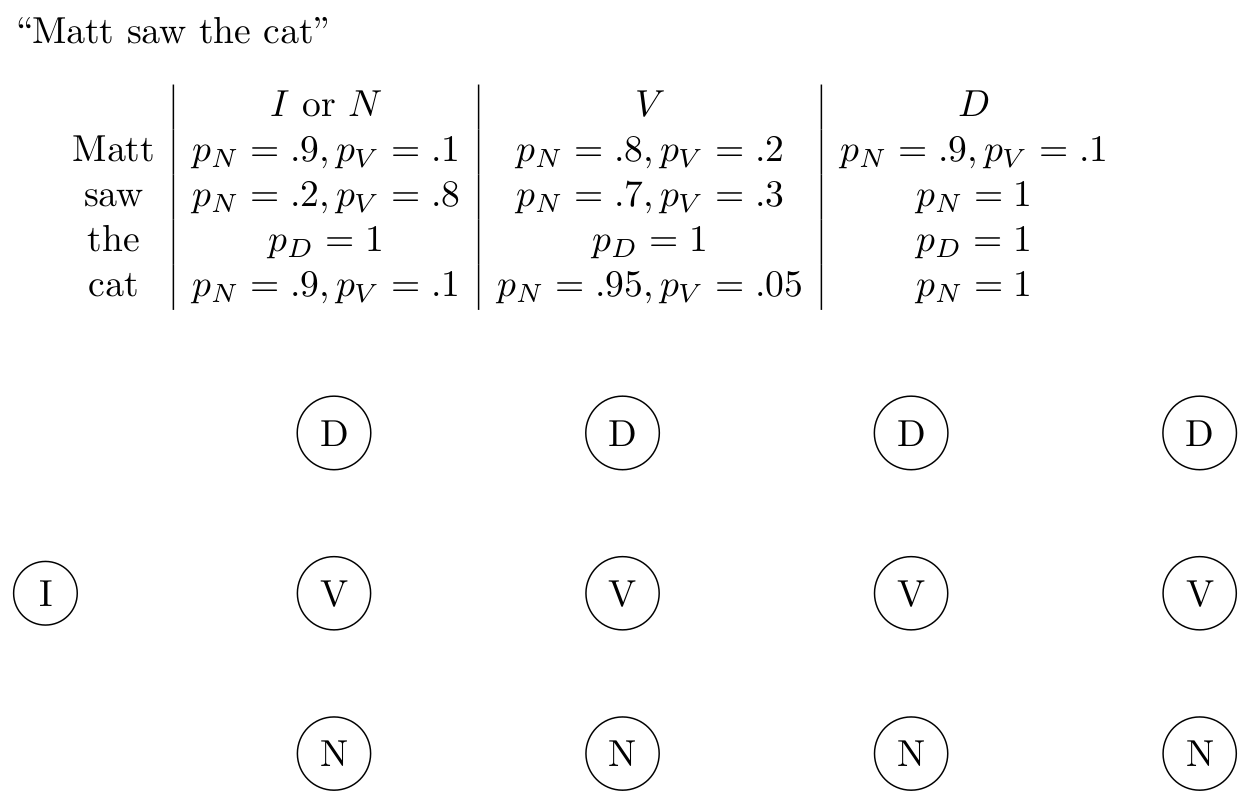
\includegraphics[width=11cm]{fig/1.png}}
\end{frame}

\begin{frame}{Алгоритм Витерби}
\centerline{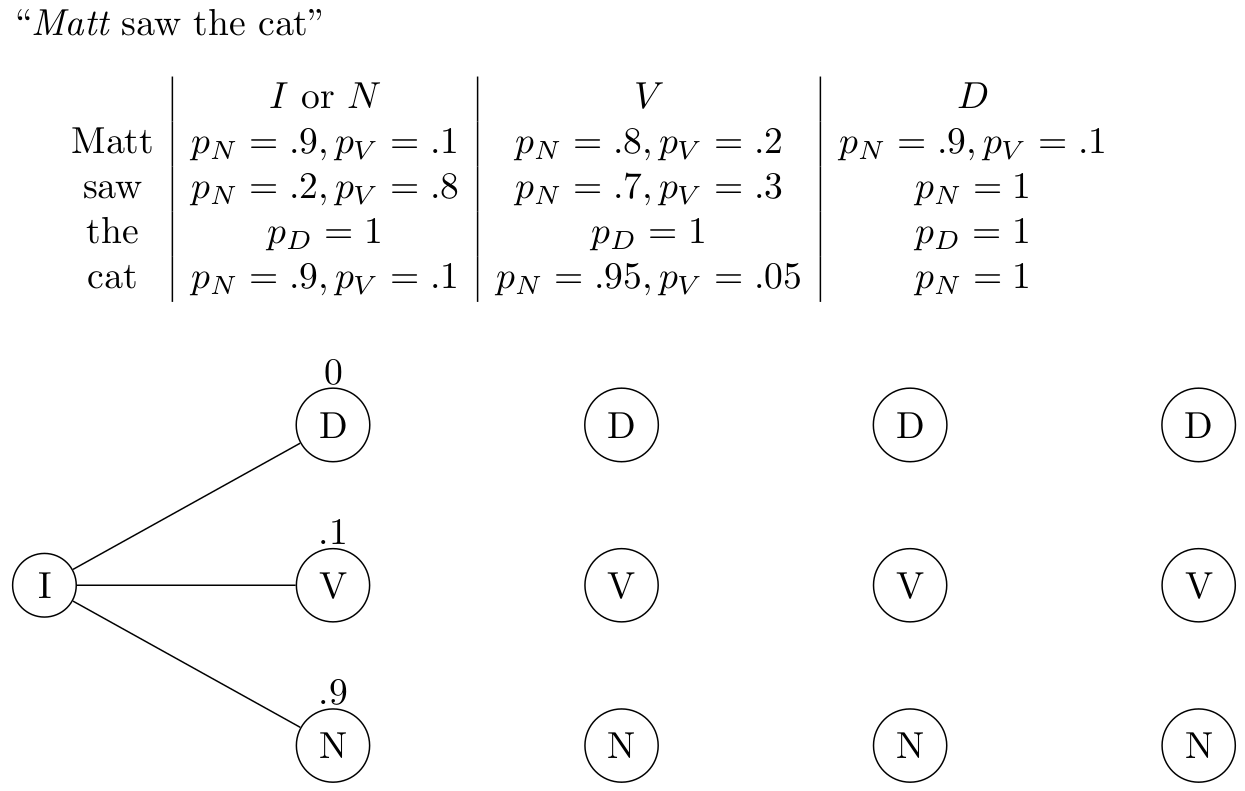
\includegraphics[width=11cm]{fig/2.png}}
\end{frame}

\begin{frame}{Алгоритм Витерби}
\centerline{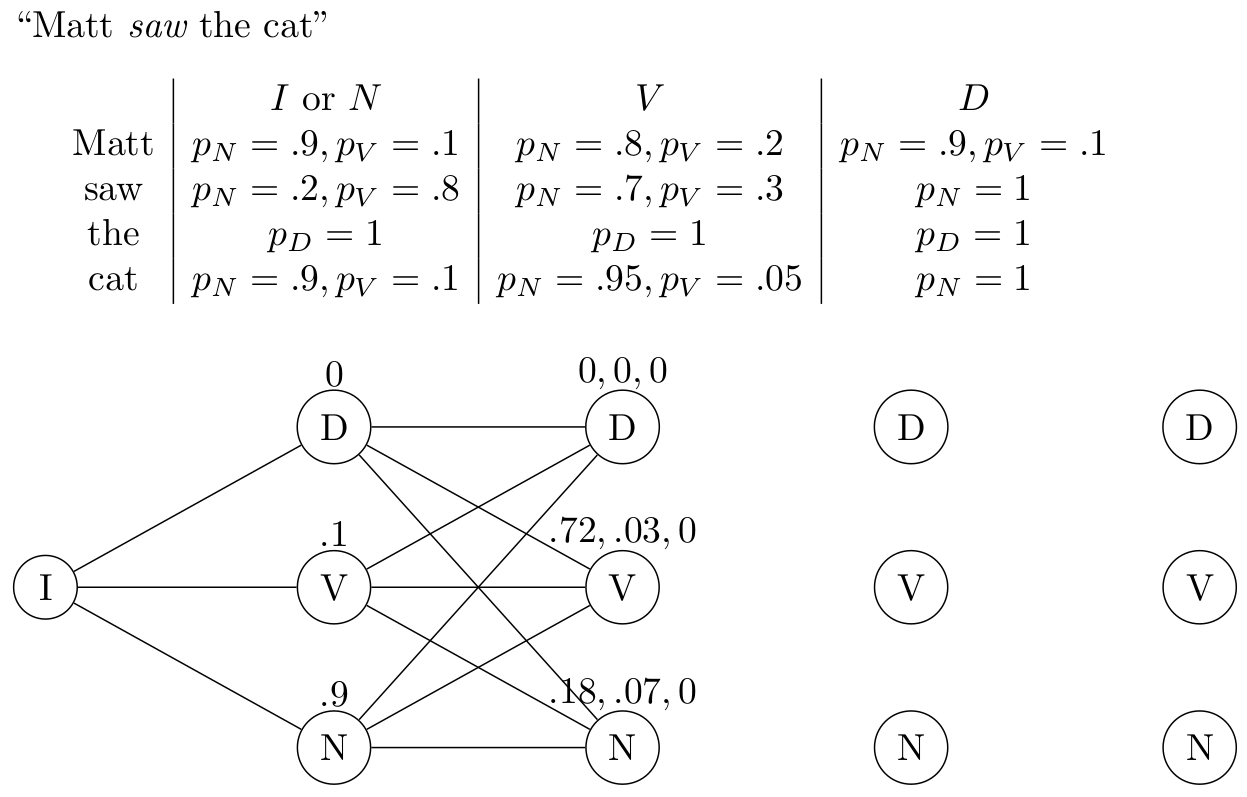
\includegraphics[width=11cm]{fig/3.png}}
\end{frame}

\begin{frame}{Алгоритм Витерби}
\centerline{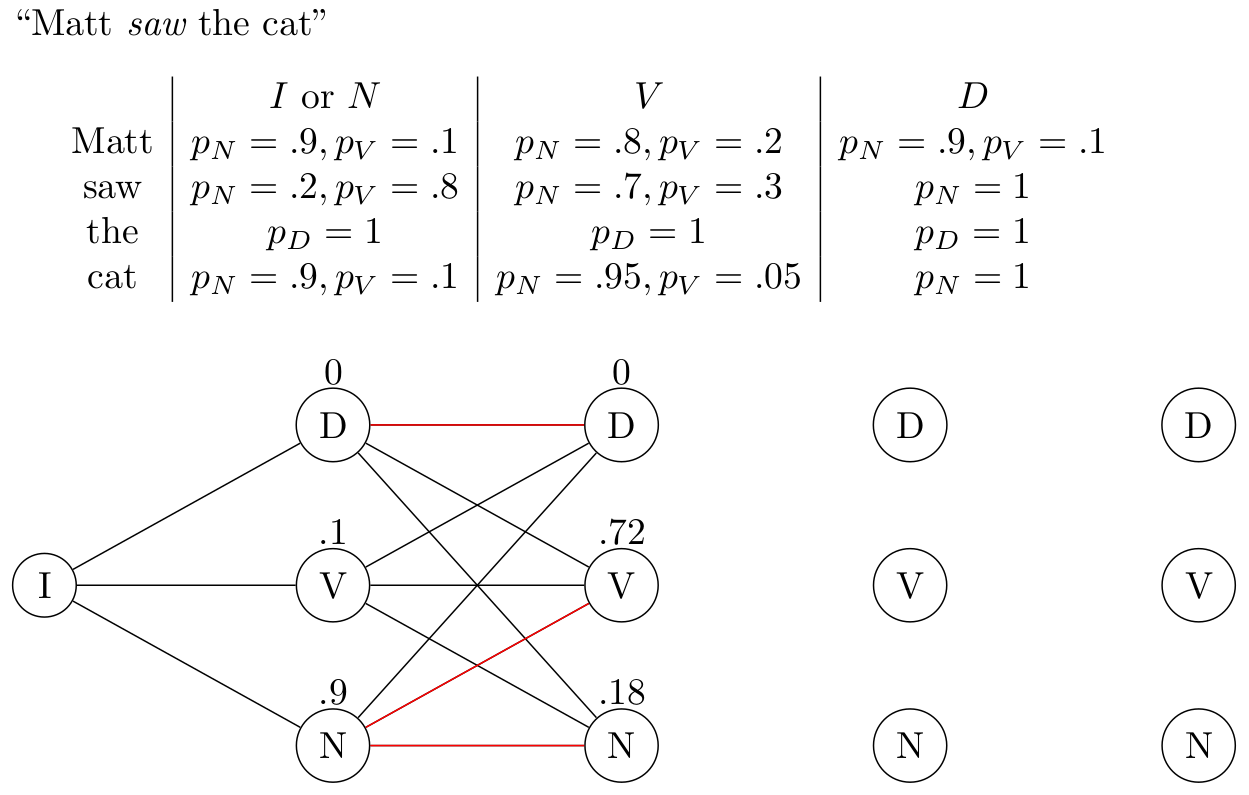
\includegraphics[width=11cm]{fig/4.png}}
\end{frame}

\begin{frame}{Алгоритм Витерби}
\centerline{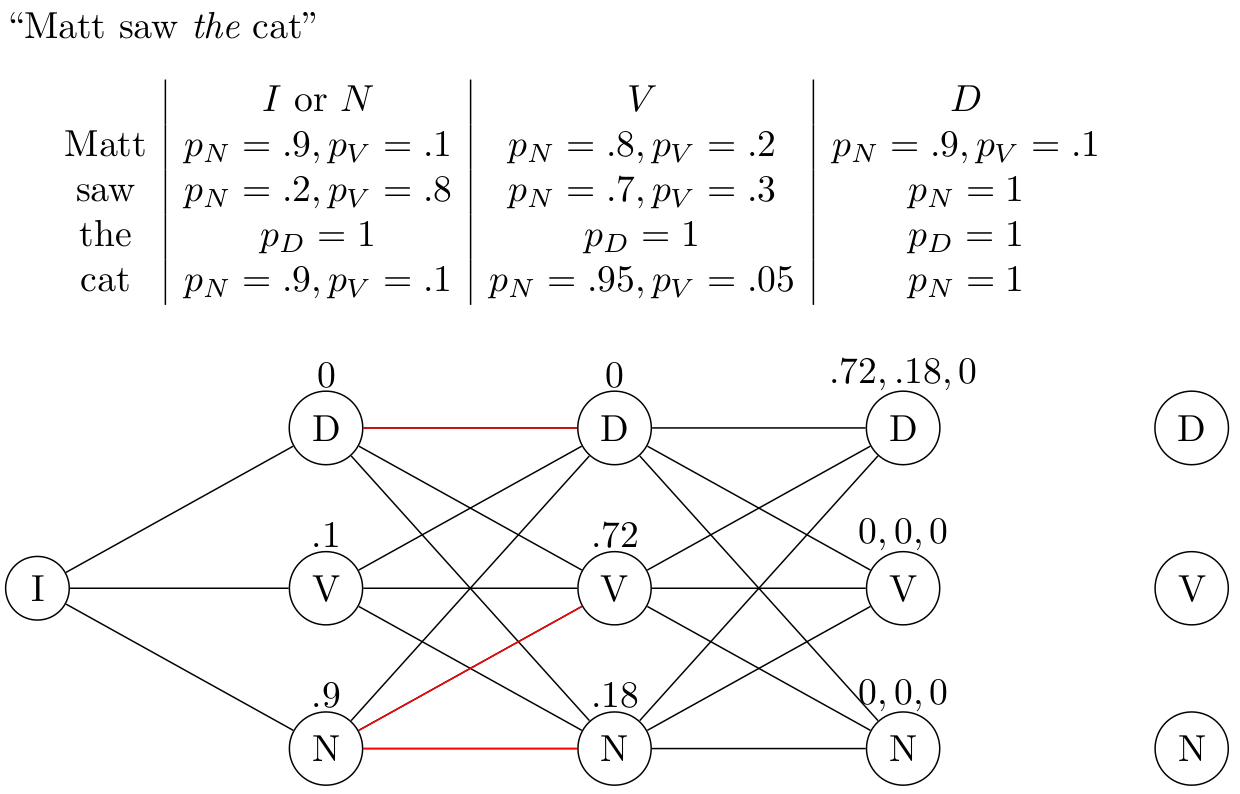
\includegraphics[width=11cm]{fig/5.png}}
\end{frame}

\begin{frame}{Алгоритм Витерби}
\centerline{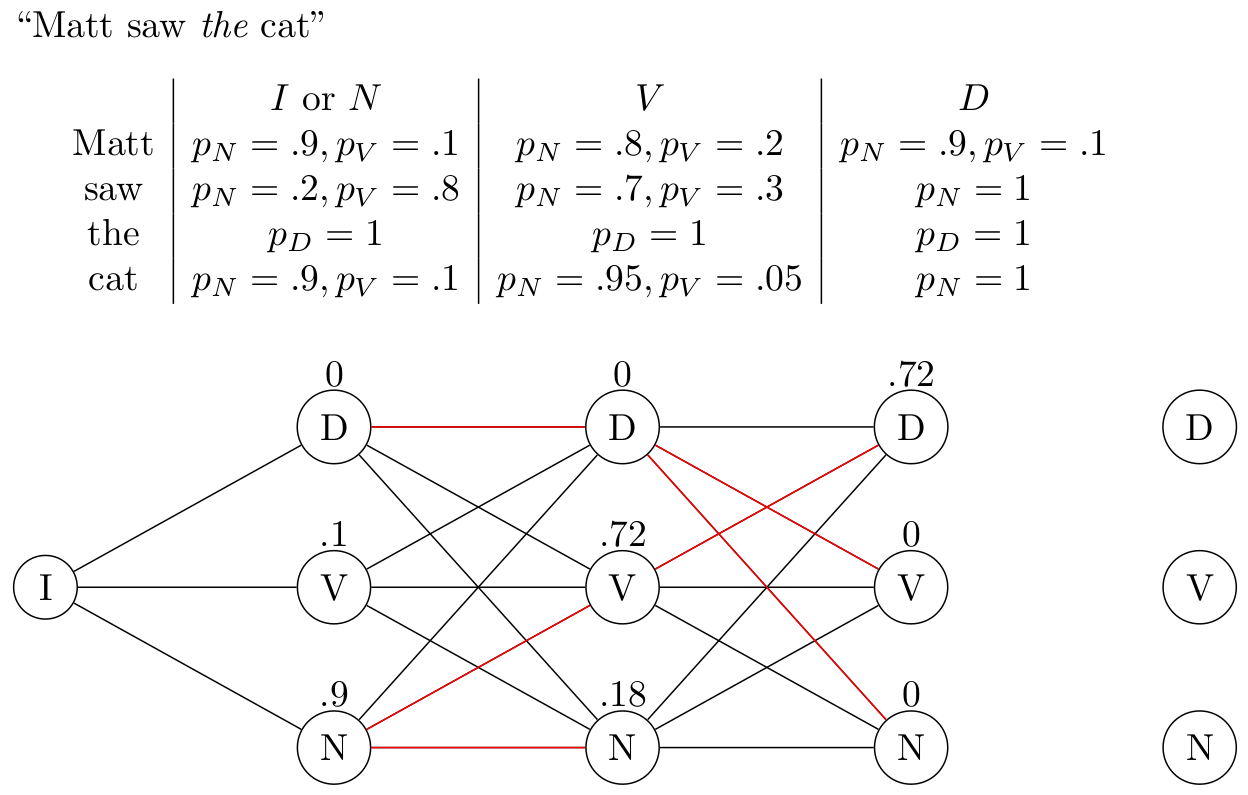
\includegraphics[width=11cm]{fig/6.png}}
\end{frame}

\begin{frame}{Алгоритм Витерби}
\centerline{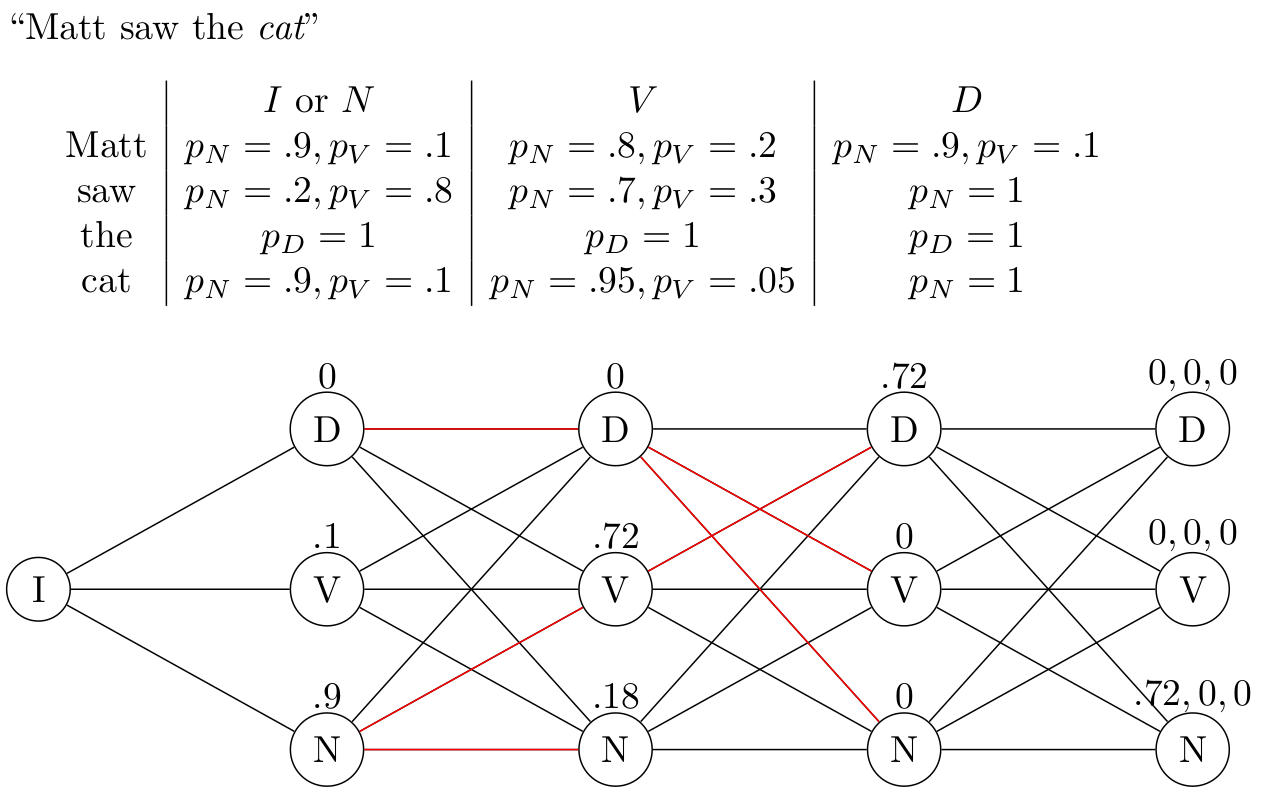
\includegraphics[width=11cm]{fig/7.png}}
\end{frame}

\begin{frame}{Алгоритм Витерби}
\centerline{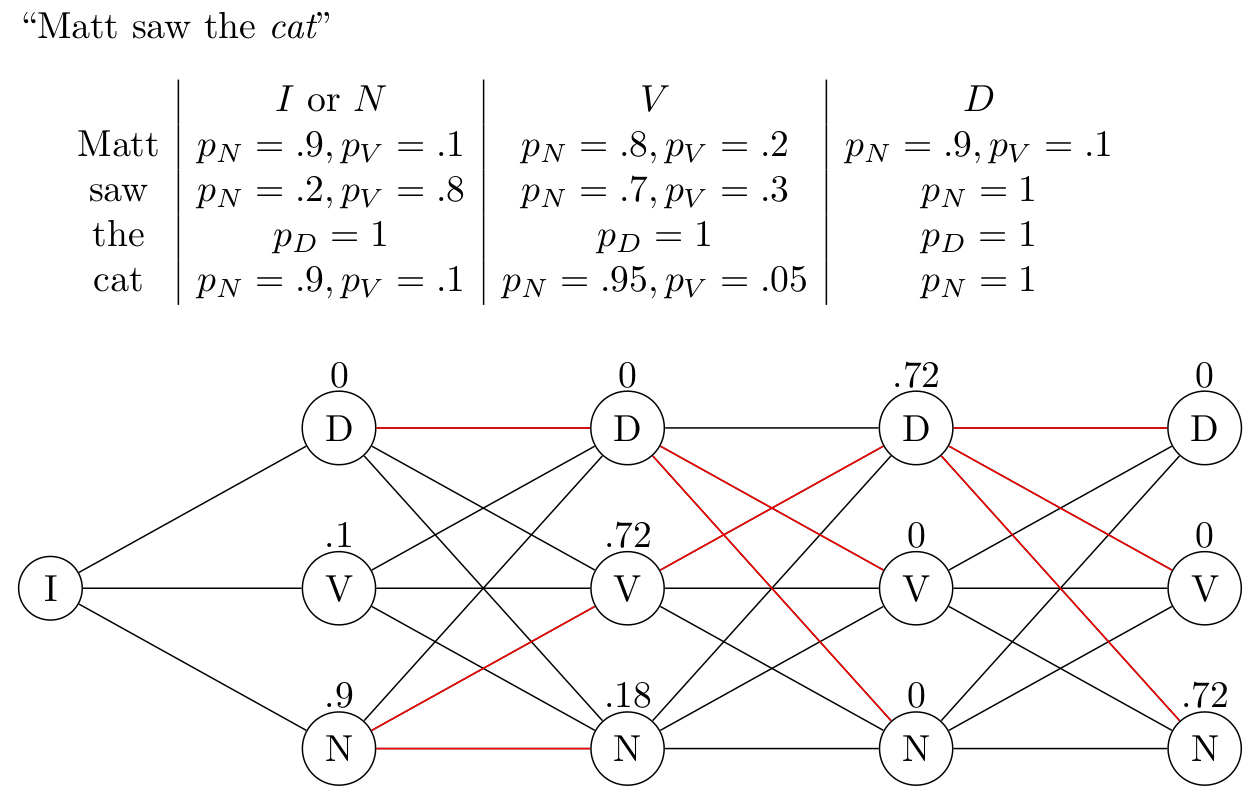
\includegraphics[width=11cm]{fig/8.png}}
\end{frame}

\begin{frame}{Алгоритм Витерби}
\centerline{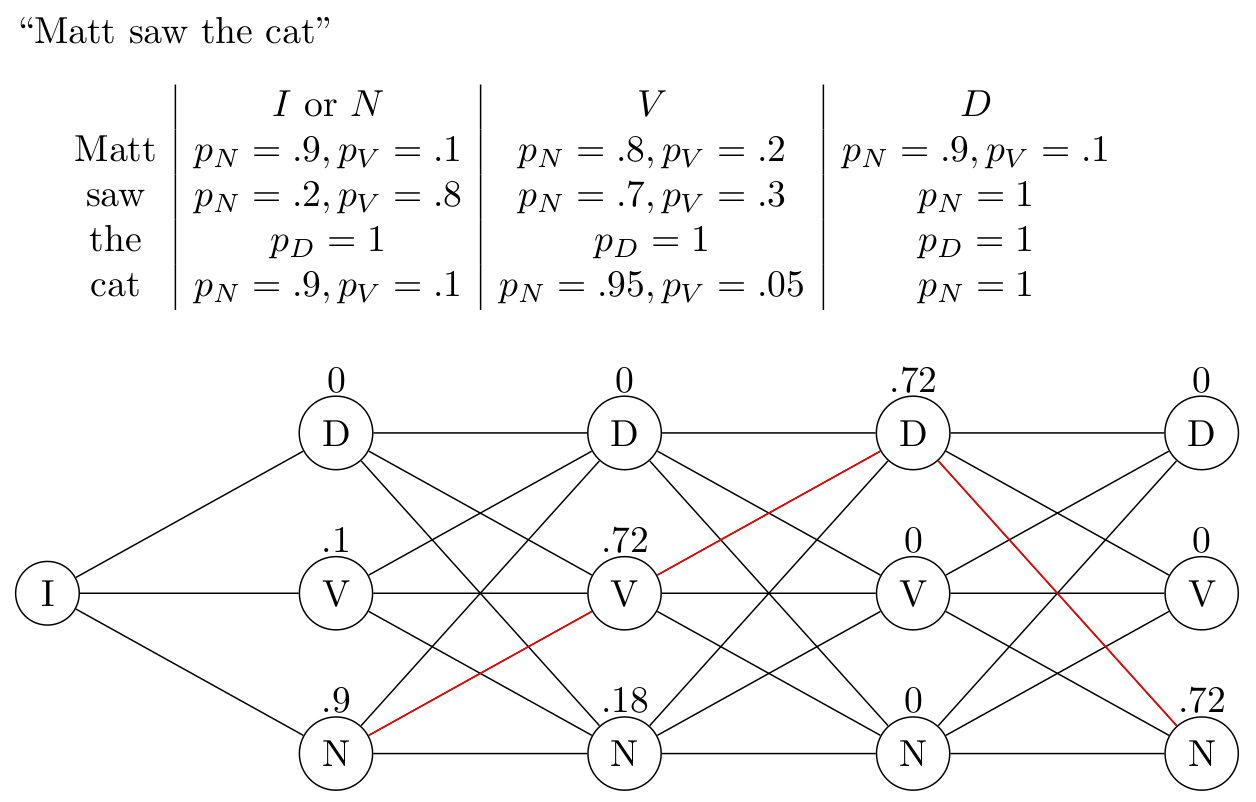
\includegraphics[width=11cm]{fig/9.png}}
\end{frame}

\begin{frame}{Резюме}
Если ответы $S$ даны (\textbf{обучение с учителем}), просто применяем алгоритм \textbf{Generalized Iterative Scaling}.\\
.\\
Если ответов нет (\textbf{обучение без учителя}), можно применить EM-алгоритм:
\begin{itemize}
\item Задать начальное приближение для $\lambda$.
\item E-шаг: вычислить вероятности ответов алгоритмом Витерби, используя $p_\lambda(s|o)$; посчитать $F^{i,s}$.
\item M-шаг: обновить переходные вероятности алгоритмом GIS.
\end{itemize}
\end{frame}

\end{document}
